% Specify IEEETran format with 10pt format, 'technote'??
\documentclass[10pt,letter,draftclsnofoot,onecolumn]{IEEEtran}
% other options...oneside,twoside,landscape,letterpaper,a4paper,etc.

\usepackage{anysize}
\usepackage{graphicx}
\usepackage{hyperref}
\usepackage{listings}
\usepackage{import}
\usepackage{color}
\usepackage{makeidx}
\usepackage[utf8]{inputenc}
\usepackage{float}
\usepackage{caption}

\usepackage{setspace}
\usepackage[margin=0.75in]{geometry}

\makeindex

\import{./}{stylin.sty}
\begin{document}

\newcommand\name{Spiel}

%
% Header
%
\title{Team 41-A (Checkmates) Project Requirements}
\author{Benjamin Friedman, Calvin Gagliano, Alex Grejuc, Kai Gay\\
Team Name: Checkmates \\
CS 461\\
Fall 2019\\
}

% Section Ordering
%\section{...}
    %\subsection{...}
        %\subsubsection{...}
            %\paragraph{...}
                %\subparagraph{...}

\begin{titlepage}
        \maketitle
        
        % turns of page numbering from here on out (until \pagenumbering used again before mainmatter)
        \pagenumbering{gobble}

        \begin{singlespace}
        \begin{abstract}
            This project requirements document describes a domain specific language (DSL) which middle school students will use to develop and understand algorithms. This document outlines the purpose, scope and practical application of this product, which is named \name. Functionality, characteristics, and other descriptive aspects are also detailed to describe the means by which this software product will accomplish our goals. We outline specific requirements that this software product must adhere to. These include what external interfaces we plan to use, requirements for usability, requirements for performance, and constraints on the design of \name. We will use the aforementioned items to judge whether \name is complete or incomplete. We will also include a reflection on how effective \name is at accomplishing its intended goals in its released form. In addition, the client (Dr. Martin Erwig) will set expectations that will be a factor in determining whether the final product is complete, as it should match (within reason) what the client originally intended it to be.
        \end{abstract}
        \end{singlespace}
\end{titlepage}
 
\begin{singlespace}

\tableofcontents
\newpage

% turns back on page numbering, resetting page count to 1 (used to put numbering back after \pagenumbering{gobble} above)
\pagenumbering{arabic}

% 1.
\section{Introduction}
    \subsection{Purpose}
        The purpose of this project is to allow for students to learn core computer science concepts through a fun and intuitive interface. As such, keeping the complexity low while still providing precision is a key goal for this project, as this will likely be the intended audience's first introduction to programming.
    \subsection{Scope}
        We will be producing \name, an educational tool intended for the specification and play of two dimensional board games by middle school students. We limit this tool to the language itself, a syntax-directed editor for writing programs in the language, a translator for the language, and a game engine which allows users to play the game and view a game's trace. The intent is not to make a high performance graphical rendering system or artificial intelligence game-playing system. However, if time permits, these are possible extensions to our core project. Additionally, we do not intend to create a language that can describe any board game. Rather, the project will be limited to a subclass of games that are deemed pedagogically interesting and share a similar collection of features that are implementable. The games will be
        \begin{enumerate}
            \item Abstract -- they require no significant art skills, and the pieces do not signify anything concrete
            \item Strategic -- each player takes one turn at a time
            \item Games of perfect information -- all information is visible to all players
            \item Played on a rectangular grid -- reasoning about a grid is simple enough for middle school students
        \end{enumerate}
        By restricting the domain of the language in this way, we will be able to provide a simpler language.
        
    \subsection{Product Overview}
         This product, \name, is to be a software based solution to assist middle school students (ages 11 - 14) in their comprehension of early computer science concepts. This will be mainly accomplished by the primary product: a domain specific language (DSL) that describes simple board games and an interpreter for the DSL. Writers of the DSL will be able take elements from one game that is represented in the language and apply it to another. The language will be written in Haskell, a purely functional programming language. The primary product may be accompanied by a syntax-directed editor for the language or an artificially intelligent agent that attempts to play the described games. Both of these potential sub-products will be created in order to provide a richer learning experience to \name's audience. The product will be served primarily as a web-based application, but is also capable of being distributed as a stand alone executable as well.
    \subsubsection{Product Perspective}
        Our product, \name, is related to the products 'Zillions of Games' and distantly related to 'Scratch'\cite{scratch}. Zillions of Games provides a language that is intended to purely express as many games as possible in a singular language. Our product differs by our focus on board games specifically, and to use the language as a means to teach basic understanding of algorithms. Ideally, the restriction of focus will result in a simpler language. In addition, Scratch also seeks to teach an understanding of coding, including algorithms, but through a block-based approach. This is different than what we are attempting here.
        
        
        This software will be designed with the intent to be understandable, usable, and educational for 7th to 8th grade students who are in middle school. Although this is the primary audience for this software based product, the product should also be usable by groups in older categories of users such as the teachers who will teach it to the students. Potentially younger students may be interested in learning as well.
        
        
        For a system interface, our product will be available to most modern computers systems (i.e. Windows 10, Mac, Linux Ubuntu, etc.). The potential syntax-directed editor (secondary product) provide a graphical user interface (GUI) for easier interaction with our language. It might also provide a way to visualize playing of the described game (i.e. the user's program). All user interface components should be simple enough for a 7th grader to use to develop an understanding of our product. Our hardware interfaces will consist of the standard peripherals needed to interact with computers: a mouse, keyboard, and a monitor. Our software interface will consist of a host language by which our developed DSL will be implemented in. Communications interfaces will be akin to our hardware interfaces where the monitor will be used to communicate information back to the user. Constraints on memory will likely not be an issue, as we don't expect to be calculating large numbers of possible moves or storing large quantities of data of any sort. 
        
        
        Considering all of this, product operations will be based on a modern computer platform and with a standard means of interacting with the hardware (mouse, keyboard, and monitor). Operations will consist primarily of using the product to display and take input from a user trying to play a board game as described by various rules. As it stands, no data will be stored beyond an active session. This is due to concerns on storing and handling data of underage individuals, which may lead to concerns with regards to their privacy. Also, there is no important reason to store any sort of data. Instead, we intend to reflect on performance on tasks before and after using our product as a means to directly measure its effectiveness. This may be later changed if the group comes to a consensus on how to handle user data appropriately with our client. As it stands, no backup and recovery options will be needed, as no data retention will be put into place.
        
    \subsubsection{Product Functions}
        The domain specific language will be able to precisely describe the rules and format of customized board games. The translator will be able to read this language, translate it to a host language, and use the host language's translator to allow play of the board game. The board game that the user can play is equivalent to the user's program. The DSL should be usable without any knowledge of how the translator works. In addition, the editor will allow for friendly and interactive editing of this language, and the translator should provide helpful improper-use messages (syntax error, run-time, etc.). 
    \subsubsection{User Characteristics}
        The users of this product will include but will not be limited to students of Linus Pauling Middle School and instructors/researchers in the computer science education field. Specifically, the first students to use this product will be in the seventh grade, and the teachers helping students who are physically present in the classroom. This product can also be used by the client and other educators at academic institutions who wish to teach the product.
        
    \subsubsection{Limitations}
        This software product will be limited by the inherent understanding of the board games that 7th graders can understand. If the user cannot understand any board games that can be played using this product or can only understand them in a limited fashion, then this product will not be of use to them. In addition, those who are visually impaired will be unable to use this software product, as it will require vision to navigate the visual interface. Furthermore, an assumption of basic computer literacy is being made since users who cannot operate a computer via a keyboard, mouse, and a monitor will be unable to utilize this product. Retention of usage statistics by users will not be put in place, as there are significant regulatory implications of handling data for 7th grade students (this is also mentioned in the product perspective section above, and may change).
        
    \subsection{Definitions}
        \begin{itemize}
            \item Domain specific language (DSL): A computer based language that is designed with an emphasis for use in a particular context or application.
        \end{itemize}
    
% 2
\section{Specific Requirements}
    \subsection{External Interfaces}
        All of our subsystems will utilize a visual interface by means of a standard computer monitor (present on most laptops and desktops). Input will be enabled through use of a keyboard and mouse, and in other cases it may be enabled through a touch screen (substituting as both a mouse and a keyboard).
        
        The initial input to our software system is a program written in the language \name through a text file. This will be done in an editor of the user's choice or through our syntax-directed editor. This text file will be provided to our translator service, running as a backend web application, which will then produce a game. This game will finally be playable by users through the keyboard or touch interface by requesting input from the users and outputting a graphical representation of the game in their browser
        
    \subsection{Functions}
        The translator takes a description of a board game in our DSL and allows for execution of the complete game according to the rules described. This will include handling player turns, keeping track of previous moves, providing informative error messages when a move is not permitted, and determining a winner. When checking the validity of inputs, the translator will produce an error message detailing the syntax error and its location in the source program and then terminate execution. 
        
        The editor will allow for varying complexity of levels beginning with a "template" type system and ending with total freedom, as the user progresses through learning the language. 
        
        Our system will function as follows: a user will specify a program in our DSL, \name. They may do so by supplying text produced in an editor of their choice or through our syntax-directed editor. Once this program is complete, the user will request their program to be translated. If the program contains syntax errors, the translator will produce an error message and stop executing. The user may then attempt to fix their program and translate again. If translation succeeds, a game will be produced. Users will then play this game by providing inputs to prompts.
        
    \subsection{Usability Requirements}
        The software product must have the following usability requirements at minimum:
        \begin{enumerate}
            \item the DSL should be able to describe and make Tic-Tac-Toe, Connect 4, and other similar board games
	        \item the DSL should require no programming experience to understand and to use
	        \item the DSL should be usable with only a previous understanding of how to play one of the board games listed above
	        \item instructions for one game written in the DSL should also work in another similar board game (but may not have the same result)
	        \item users should be able to articulate patterns pertaining to 'how to play' and 'how to win' for one or more board games in the DSL after play
        \end{enumerate}
    \subsection{Performance Requirements}
        The software product must have the following performance requirements at minimum:
        \begin{enumerate}
            \item the software should run on most modern computing systems that are capable of running Haskell
            \item the software should not unreasonably consume resources in a way that makes it unusable
            \item the visual aspect of this software must remain remain responsive in all cases
            \item The interface should be functional in both a web-based and desktop based context.
        \end{enumerate}
        
        All of the games within the scope of this project are played turn-by-turn so simultaneous users will not be supported. 
    \subsection{Design Constraints}
        The software product will have the following design constraints:
        \begin{enumerate}
            \item It will be written in a host language (Haskell at this time), unless another language or combination of languages is approved by the group and client
            \item It will be written and designed to work on a desktop environment
            \item It should require no programming experience to utilize
            \item Should be accessible to a student in middle school in terms of technical competence.
            \item Must be legally acceptable for academic use with middle school students
        \end{enumerate}
    \subsection{Software System Attributes}
        The software must be reliable: user tests should reveal no errors, and unit tests should be written for all major features. If the end product is hosted online, the software should be readily available without much technical knowledge. The product should be relatively reliable, meaning that it must be stable enough to allow a user to complete an intended duration of use. The product will have no reset or restart functionality, as it will be setup to work for any of the board games we choose. From this point, the user then attempts to 'play' the game being described through our visual interface.
        
        
        % security...
        Security implications with our product will be minimal as we intend to collect no data for storage nor connect with other software, devices, or systems during use. Security implications that we could face would be related to unintended manipulation or misuse of our product in order to achieve a malicious intent. This would most likely include targeting a separate process within the same system. To circumvent these kinds of attacks, we intend to ensure data integrity of the input provided such that our program cannot be used in a way that can lead to unintended usage or illegal behavior. Additional security concerns are present with the usage of a web-based system, which will be sending and receiving data from a remote source. As such, the data will need to be secured in a fashion to prevent tampering and inspection by an unauthorized user.
        
        
        % maintainability
        The product will be built for maintainability by following these guidelines:
        \begin{itemize}
            \item proper documentation must be in place for the overarching structure of our product, allowing new and existing developers to understand the layout of the program
            \item proper testing must be in place for all functionality that is reasonably possible, and to cover as many branches as reasonably possible (reasonably meaning within our resources, physical capability, and allotted time)
            \item components of the product will only be designed and developed until they fulfill the requirements of them, either indicated by documentation or testing driven development (TDD)
            \item referencing the guideline above, extraneous functionality will be trimmed, unless extenuating circumstances (that the team agrees on applies)
        \end{itemize}
        
        
        % portability
        The product will built to be reasonable portable for at least one platform (Windows, Mac, Linux). Portability may be limited by the graphical interface of our product, which may depend on using system specific implementations. However, barring this our product should be platform independent, with independence qualifying capability of usage on Windows, Mac, and Linux platforms. In the web-based version our application will be functional on Firefox, Safari, Chrome, and Edge, allowing for a high degree of portability.
    \subsection{Supporting Information}
        There are no current supporting documents that we are ready to formally list. Documents that we collectively agree upon will be added into this section accordingly.

% 3
% Believe this is definition of done, what constitutes completeness of the software product
\section{Verification}
    \iffalse
    Verification will constitute meeting and/or exceeding the aforementioned stated performance and usability requirements, all while adhering to the design limitations we have imposed on this project. In addition, verification of the product is also contingent on it being practically usable and demonstrable as an educational aid. Assuming these requirements have been met, verification according to our group's collective definition of done will have been met.
    \fi
    
    % possible verification points...delete these once verification is done below
    
    % The domain specific language will be able to precisely describe the rules and format of customized board games.
    
    % The users of this product will include but will not be limited to students of Linus Pauling Middle School and instructors/researchers in the computer science education field.
    
    % This software product will be limited by the inherent understanding of the board games that 7th graders can understand.
    
    % All of our subsystems will utilize a visual interface by means of a standard computer monitor
    
    % The translator takes a description of a board game in our DSL and allows for execution of a complete game, according to the rules described
    
    % there will also be an editor that will allow the user to experience varying levels of complexity
    
    % performant given a modern operation system, 8 GB of Ram, and a standard OS (Windows,Mac,Linux)
    
    % adhere to our above stated design specifications, usable by students, written in a host language etc...
    
    % well tested, secure, maintainable and portable across major OSs

    We will verify our software through a test suite and feedback from our client. We do not need to verify the external interfaces given that a keyboard and mouse interface are supplied by the computer itself. We will verify the functions of the software through a test suite and an integration step in which we will validate the sequence of operations specified above can be carried out successfully. We will verify the usability requirements through self-assessment and our client's feedback, but not through user studies, as this is beyond the scope of our work. Given that our project does not have strict performance requirements, we will only informally verify that the software does not have significant latency problems. We do not intend to use a logical database so there is no need to verify this portion. We will verify the design constraints and software system attributes by checking that each point specified in the relevant sections has been met.    
% 4
\section{Appendices}
    \subsection{Assumptions and dependencies}
        We assume that the product will be used from a non-mobile computer through a web interface.
    \subsection{Acronyms and abbreviations}
        \begin{itemize}
            \item DSL: Domain specific language
            \item GUI: Graphical user interface 
            \item TDD: Test-driven development 
        \end{itemize}{}

% 5

\newpage
\section{Gantt Chart}


The following outlines the general layout and flow of the tasks in our project for this year.

\begin{figure}[H]
  \centering
  \captionsetup{justification=centering}
    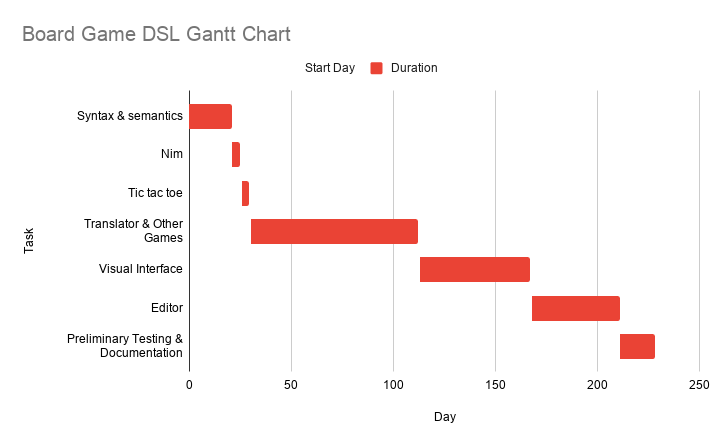
\includegraphics[width=1.0\textwidth,keepaspectratio]{./img/gantt}
    \caption{A Gantt chart specifying a timeline and the dependencies of our milestones}
\end{figure}

%%%%%%%%%%%%%%%%%%%%%%%%%%%%%%%%%%%%%%%
%\bibliographystyle{IEEEtran}
%\bibliography{refs} % your .bib file

\begin{thebibliography}{99}
%\bibitem{pa} H.~Partl:\emph{German \TeX},TUGboat Volume~9, Issue~1 (1988)
\bibitem{scratch} "Scratch- Imagine, Program, Share", \emph{Massachusetts Institute of Technology}. Oct. 2019. https://scratch.mit.edu/. Accessed Oct. 10th, 2019.
\end{thebibliography}
%%%%%%%%%%%%%%%%%%%%%%%%%%%%%%%%%%%%%%%

\end{singlespace}
\end{document}8